% Z[sqrt(-5)] as a lattice in C, with the ideals P=(2,1+sqrt(-5)) and (2).
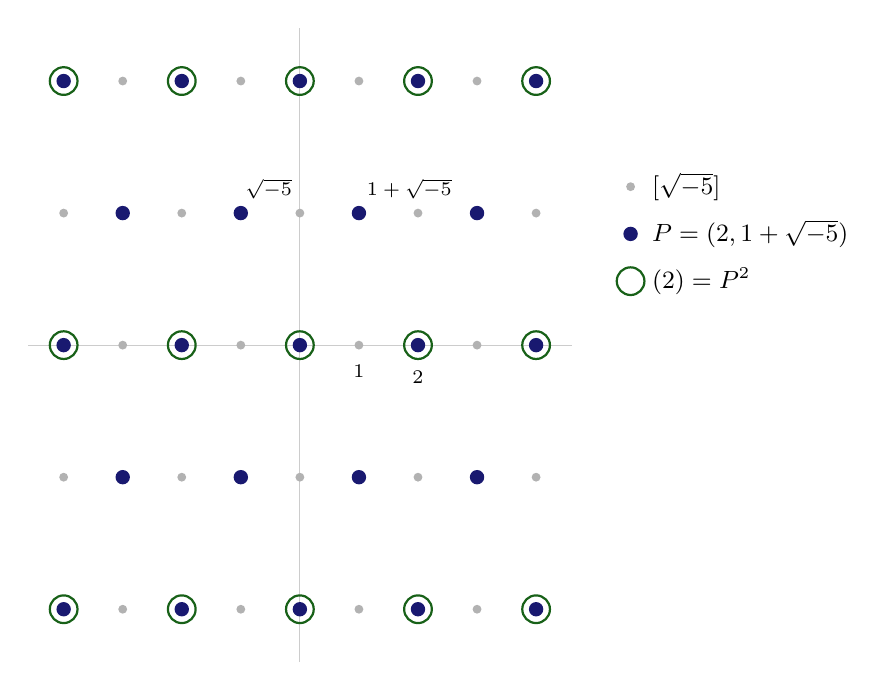
\begin{tikzpicture}[x=0.75cm,y=1.677cm]
  \draw[gray!40] (-4.6,0) -- (4.6,0) (0,-2.4) -- (0,2.4);
  \foreach \a in {-4,...,4} \foreach \b in {-2,...,2} {
    \pgfmathtruncatemacro{\inP}{mod(abs(\a+\b),2)==0}
    \pgfmathtruncatemacro{\inTwo}{(mod(abs(\a),2)==0) && (mod(abs(\b),2)==0)}
    \ifnum\inTwo=1 \draw[ForestGreen!70!black,thick] (\a,\b) circle (5pt); \fi
    \ifnum\inP=1 \fill[MidnightBlue] (\a,\b) circle (2.6pt);
    \else \fill[gray!60] (\a,\b) circle (1.6pt); \fi
  }
  \node[below,font=\scriptsize] at (1,-0.08) {$1$};
  \node[above left,font=\scriptsize,fill=white,inner sep=1pt] at (-0.08,1.08) {$\sqrt{-5}$};
  \node[above right,font=\scriptsize,fill=white,inner sep=1pt] at (1.08,1.08) {$1+\sqrt{-5}$};
  \node[below,font=\scriptsize] at (2,-0.12) {$2$};
  \begin{scope}[shift={(5.6,1.2)},font=\small,y=1cm]
    \fill[gray!60] (0,0) circle (1.6pt); \node[right] at (0.2,0) {$\Z[\sqrt{-5}]$};
    \fill[MidnightBlue] (0,-0.6) circle (2.6pt); \node[right] at (0.2,-0.6) {$P=(2,1+\sqrt{-5})$};
    \draw[ForestGreen!70!black,thick] (0,-1.2) circle (5pt); \node[right] at (0.2,-1.2) {$(2)=P^2$};
  \end{scope}
\end{tikzpicture}
